% Document setup
\documentclass[12pt]{article}
\usepackage[margin=1in]{geometry}
\usepackage{fancyhdr}
\usepackage{lastpage}

\pagestyle{fancy}
\lhead{Richard Whitehill}
\chead{PHYS 804 -- HW \HWnum}
\rhead{\duedate}
\cfoot{\thepage \hspace{1pt} of \pageref{LastPage}}

% Encoding
\usepackage[utf8]{inputenc}
\usepackage[T1]{fontenc}

% Math/Physics Packages
\usepackage{amsmath}
\usepackage{amssymb}
\usepackage{mathtools}
\usepackage{physics}
\usepackage{siunitx}

\AtBeginDocument{\RenewCommandCopy\qty\SI}

% Enumeration/itemize
\usepackage{enumitem}
\newenvironment{parts}
{\begin{enumerate}[label=\textbf{(\alph*)},leftmargin=*,itemsep=-10pt]
}{\end{enumerate}}

% Reference Style
\usepackage{hyperref}
\hypersetup{
    colorlinks=true,
    linkcolor=blue,
    filecolor=magenta,
    urlcolor=cyan,
    citecolor=green
}

\newcommand{\eref}[1]{Eq.~(\ref{eq:#1})}
\newcommand{\erefs}[2]{Eqs.~(\ref{eq:#1})--(\ref{eq:#2})}

\newcommand{\fref}[1]{Fig.~\ref{fig:#1}}
\newcommand{\frefs}[2]{Figs.~\ref{fig:#1}--\ref{fig:#2}}

\newcommand{\tref}[1]{Table~\ref{tab:#1}}
\newcommand{\trefs}[2]{Tables~\ref{tab:#1}-\ref{tab:#2}}

% Figures and Tables 
\usepackage{graphicx}
\usepackage{float}
\usepackage[font=small,labelfont=bf]{caption}

\newcommand{\bef}{\begin{figure}[h!]\begin{center}}
\newcommand{\eef}{\end{center}\end{figure}}

\newcommand{\bet}{\begin{table}[h!]\begin{center}}
\newcommand{\eet}{\end{center}\end{table}}

% tikz
\usepackage{tikz}
\usetikzlibrary{calc}
\usetikzlibrary{decorations.pathmorphing}
\usetikzlibrary{decorations.markings}
\usetikzlibrary{arrows.meta}
\usetikzlibrary{positioning}
\usetikzlibrary{3d}
\usetikzlibrary{shapes.geometric}

% tcolorbox
\usepackage[most]{tcolorbox}
\usepackage{xcolor}
\usepackage{xifthen}
\usepackage{parskip}

\newcommand*{\eqbox}{\tcboxmath[
    enhanced,
    colback=black!10!white,
    colframe=black,
    sharp corners,
    size=fbox,
    boxsep=8pt,
    boxrule=1pt
]}

% problem-solution macros
% \usepackage{adjustbox}
\usepackage{changepage}

\newtcolorbox{probbox}[1][]{
    breakable,
    enhanced,
    boxrule=0pt,
    frame hidden,
    borderline west={4pt}{0pt}{green!50!black},
    colback=green!5,
    before upper=\textbf{Problem #1) \,},
    % \textbf{Problem #1 \ifthenelse{\isempty{#1}}{}{: #1} \\ },
    sharp corners,
    parbox=false
}

% \newtcolorbox{ProblemBox}[1][]{%
%   breakable,
%   enhanced,
%   colback=black!10!white,
%   colframe=black,
%   title={\large #1 \hfill}
% }
\newcommand{\prob}[2]{
\begin{probbox}[#1]
#2
\end{probbox}
}

\newenvironment{solution}{\begin{adjustwidth}{8pt}{8pt}}{\end{adjustwidth}}
\newcommand{\sol}[1]{
\begin{solution}
#1
\end{solution}
}
% \textbf{#1)} #2}

% Miscellaneous Definitions/Settings
\newcommand{\reals}{\mathbb{R}}
\newcommand{\integers}{\mathbb{Z}}
\newcommand{\naturals}{\mathbb{N}}
\newcommand{\rationals}{\mathbb{Q}}
\newcommand{\complexs}{\mathbb{C}}

\setlength{\parskip}{\baselineskip}
\setlength{\parindent}{0pt}
\setlength{\headheight}{14.49998pt}
\addtolength{\topmargin}{-2.49998pt}


\def\HWnum{7}
\def\duedate{November 21, 2024}

\begin{document}

\prob{1}{

In our discussion of scattering theory in class, we made approximations that invoved assuming the limit that wavepackets became infinitely peaked (relative to what?) around some specific momenta.
It is useful to check that the approximations make sense.
Try this by considering the following generic integral
\begin{align}
    \int \dd{c} \int \dd{x} \int \dd{y} f(x) f(y) T(x,y,c) \delta(x - y)
\end{align}
with 
\begin{align}
    \int \dd{x} f^2(x) = 1
,\end{align}
and where $T(x,y,c)$ is some generally well-behaved smooth function.
If $f(x)$ is very sharply peaked (relative to the behavior of $T(x,y,c)$) around some specific value $x = r$, then we would like to replace $x \rightarrow y$ in $f(y)$.
Then we would hope we can just take $f^2(y) \rightarrow \delta(y)$ in the infinitely peaked limit.

Verify that this type of approximation makes sense by using a specific function (like a Gaussian) for $f(x)$ and a trial smooth function for $T(x,y,c)$.
Check by
\begin{parts}
    \item Evaluating the $\delta$-function first and then taking the narrow peak limit.
        Verify that you get the same thing that you would have gotten if you had just done the approximation described above from the outset.

    \item Check numerically in Mathematica that the approximation works.
\end{parts}

}

\sol{

(a) We can make the concept of a sharply peaked function inside an integral more concrete as follows.
Consider first the generic one-dimensional integral
\begin{align}
    I = \int \dd{x} g(x) f(x;x_0,\sigma)
.\end{align}
The function $f$ is ``sharply peaked'' for $x \approx x_0$ with some characteristic width $\sigma$ such that $f(x) \approx 0$ for $|x - x_0| \gg \sigma$.
Additionally, we suppose that $f$ is square integrable and that it is normalized in the usual quantum mechanical way as a probability distribution.
On the other hand, the function $g(x)$ is some generic well-behaved, smooth function of $x$ in the sense that we can split the integration domain into two pieces
\begin{align}
    I = \int_{-\infty}^{x_0 - \Delta} \dd{x} g(x) f(x) + \int_{x_0 - \Delta}^{x_0 + \Delta} \dd{x} g(x) f(x) + \int_{x_0 + \Delta}^{\infty} \dd{x} g(x) f(x)
,\end{align}
where $\Delta$ is chosen such that for $|x - x_0| > \Delta \sim \mathcal{O}(\sigma)$, $|g(x) f(x) - g(x_0) f(x_0)| < \epsilon$.
Thus, for a small enough $\epsilon$, we can neglect the two integrals away from the peak of $f$ and Taylor expand $g$ in the intermediate region:
\begin{align}
    I \approx \sum_{n=0}^{\infty} \frac{g^{(n)}(x_0)}{n!} \int_{x_0 - \Delta}^{x_0 + \Delta} (x - x_0)^{n} f(x)
.\end{align}
The smoothness of $g$ comes in here, where we suppose that the derivatives of $g$ over the interval $x \in (x_0 - \Delta,x_0+\Delta)$ are quite small such that
\begin{align}
    I \approx g(x_0) \int_{x_0-\Delta}^{x_0 + \Delta} \dd{x} f(x) \approx g(x_0) \int \dd{x} f(x)
,\end{align}
where in the last approximation we have extended our integration domain back to the entire real line, which is typically more practical for completing the integrals analytically and justifiable given that $f$ falls off rapidly in these tails by assumption.

We can apply this kind of logic to the multi-dimensional integral
\begin{align}
    I = \int \dd{c} \int \dd{x} \int \dd{y} f(x) f(y) T(x,y,c) \delta(x - y)
.\end{align}
For our first approach, we naively replace $y$ with $x$ as follows since $f$ is sharply peaked:
\begin{align}
    I = \int \dd{c} \int \dd{x} \int \dd{y} f^2(x) T(x,y,c) \delta(x - y) = \int \dd{c} \int \dd{x} f^2(x) T(x,x,c)
.\end{align}
Taking the infinitely-peaked limit, we replace $f^2$ with a delta function centered at some $x = r$ such that
\begin{align}
    I = \int \dd{c} T(r,r,c)
.\end{align}

Let us now take the slightly different approach by first integrating out the delta function:
\begin{align}
    I = \int \dd{c} \int \dd{x} f^2(x) T(x,x,c) = \int \dd{c} T(r,r,c)
,\end{align}
which is the same result we obtained in the naive approach.


(b) To check the approximation, we use a Gaussian
\begin{align}
    f(x) = \frac{1}{\sqrt[4]{\pi \sigma^2}} e^{-x^2/(2 \sigma^2)}
,\end{align}
which is properly normalized in the quantum mechanical sense.
For our test function, we use
\begin{align}
    T(x,x,c) = e^{-|x - c|}
,\end{align}
which although not necessarily a physically nice function, we can gurantee convergence for integrals over the entire real line.
Indeed, when $\sigma \rightarrow 0$, $f^2(x) \rightarrow \delta(x)$ and
\begin{align}
    \int \dd{c} T(0,0,c) = 2
.\end{align}
We can see that for the functions chosen, when $\sigma < 10$, our approximation begins converging on the value we obtain using the method of steepest descent as described in part (a).

\begin{figure}[h!tb]
    \centering
    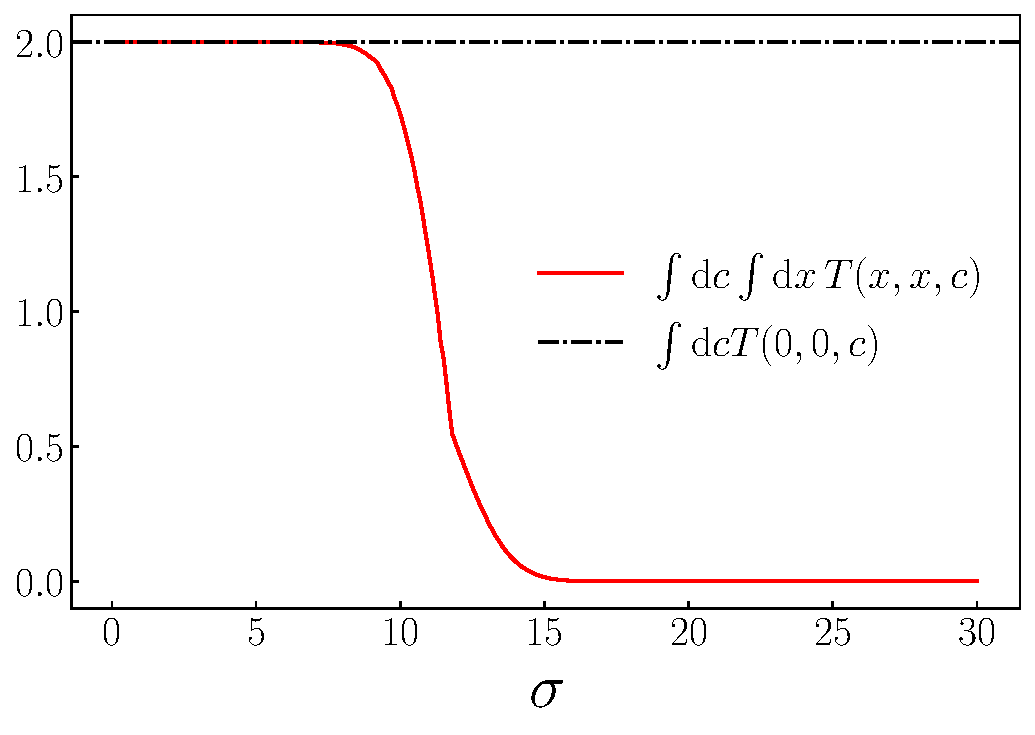
\includegraphics[width=0.7\linewidth]{prob1.pdf}
\end{figure}

}


\prob{2}{

\textbf{Reading Assignment}: Compare the way I have set up the treatment of interacting relativistic QFTs with the treatment in Weinberg's textbook (chapter 3) and Gross' textbook (chapters 9 and 3).

\begin{parts}
    
    \item Are there aspects of the logic that conflict with what I have presented? Explain.

    \item Can you identify aspects that are incomplete?

    \item Can you find other textbooks or resources that are closer to my treatment?

\end{parts}

}

\sol{

Weinberg also focuses his introduction to interacting quantum field theories through the lens of scattering, although he focuses more heavily from the onset on the $S$-matrix.
The matrix elements describe transitions of idealized particle states (i.e. eigenstates of our Hamiltonian which are not quite physical) at $t \rightarrow -\infty$ evolving into those at $t \rightarrow \infty$.
In what follows his first few sections, although Weinberg states that for a fully rigorous and formal derivation, one must consider wave-packets, he proceeds with the typical ``derivation'' of probabilities, rates, and cross-sections in a large box, which of course introduces many factors of $V$, the volume of the space, and $T$, the time-duration for which interactions are allowed occur but happily cancel in the end\footnote{It may also be notable that placing systems in boxes breaks many of the symmetries Weinberg worked so hard to explore in the previous sections.}.
After ``deriving'' the generic decay rate and cross section formulas, Weinberg discusses perturbation theory.
He first uses the Lippman-Schwinger equation to derive a formula for the $T$-matrix, which although not used in modern calculations and not being manifestly Lorentz invariant, elucidates clearly the connection between singularities of the $S$-matrix with intermediate states.
Taking a more modern approach, Weinberg then derives the Dyson series representation of the $S$-matrix\footnote{Additionally, there is a clear motivation for giving a small imaginary component to our time which exponentially damps instead of growing for large $t$.} and deduces what kind of interacting theories are manifestly Lorentz invariant.
Finally, before studying partial wave expansions and resonances, Weinberg derives the optical theorem from the unitarity of the $S$-matrix.


In chapter 9 of Gross' textbook, the $\phi^3$ theory is introduced as a playground to study interacting theories.
Previously, in chapter 3 of his textbook, Gross developed time-dependent perturbation theory in the interaction picture within the context of nonrelativistic quantum mechanics and electromagnetic interactions, although he claims that the arguments were general enough to apply within the context of quantum field theory and immediately writes the interaction picture time-evolution operator as the Dyson series.
In the next sections, Gross develops the generic formulae for decay rates and cross sections, although his work depends on the details of $\phi^3$ theory, and is not clearly immediately generalizable.
After this, Gross analyzes the amplitude and sketches how one may obtain the Feynman rules, although the discussion is far from complete.
In the remaining sections of chapter 9, Gross gives concrete examples for calculating cross sections in the lab and center-of-mass frames, demonstrates how the Yukawa potential is obtained by considering a simple particle exchange in field theory, and discusses Feynman rules for theories of the Standard Model.
While Gross' book is more complete in deriving Feynman rules and shows some interesting non-relativistic limits, the motivation for the need of Feynman rules in the first place is somewhat unsatisfying, given that it is only motivated at the level of two-point interaction in $\phi^3$ theory and made to seem plausible that such a treatment and structure holds beyond these terms.

}
    
\end{document}
